%%%%%%%%%%%%%%%%%%%%%%%%%%%%%%%%%%%%%%%%%%%%%%%%
% COPYRIGHT: (C) 2012-2015 FAU FabLab and others
% Bearbeitungen ab 2015-02-20 fallen unter CC-BY-SA 3.0
% Sobald alle Mitautoren zugestimmt haben, steht die komplette Datei unter CC-BY-SA 3.0. Bis dahin ist der Lizenzstatus aller alten Bestandteile ungeklärt.
%%%%%%%%%%%%%%%%%%%%%%%%%%%%%%%%%%%%%%%%%%%%%%%%


\newcommand{\basedir}{fablab-document}
\documentclass{\basedir/fablab-document}

% \usepackage{fancybox} %ovale Boxen für Knöpfe - nicht mehr benötigt
\usepackage{amssymb} % Symbole für Knöpfe
\usepackage{subfigure,caption}

\usepackage{marvosym} % für Briefumschlag-Symbol
\usepackage{eurosym}
\usepackage{tabularx} % Tabellen mit bestimmtem Breitenverhältnis der Spalten
\usepackage{wrapfig} % Textumlauf um Bilder
\renewcommand{\texteuro}{\euro}

\linespread{1.1}
\setlength{\parskip}{0.5em}
\date{August 2013}
\author{}
\fancyfoot[L]{kontakt@fablab.fau.de}
\title{Anleitung Buttonpresse}

\newcommand{\todo}[1]{\textbf{\color{red}{TODO: #1}}}
\begin{document}
\vbox{ % Hack, damit Überschrift nicht soviel Platz verbraucht und alles auf 1 Seite passt
\vspace{-3em}
\maketitle
\vspace{-3em}
}
\section{Vorlage}

Papiervorlage: 56mm Durchmesser außen, nutzbare Fläche etwa 42mm, dazu kommen einige Millimeter seitlicher Rand. Farbige Hintergründe bis mindestens 50mm fortsetzen, damit es keinen weißen Rand gibt!

\begin{figure}[h]
\caption{Vorlage für ein selbstgestanztes Motiv}
\begin{center}
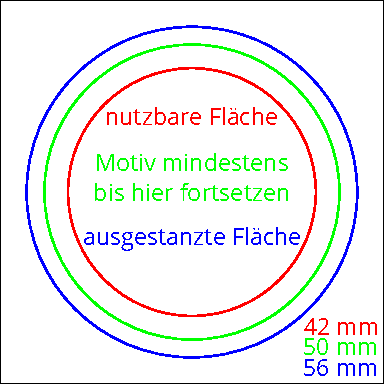
\includegraphics[scale=1]{img/motivvorlage.pdf}
\end{center}
\end{figure}

Mit der Stanze kannst du aus Papier die passenden 56mm Kreise ausstanzen. Dazu ein Stück Papier grob zuschneiden, einschieben und draufdrücken.


\section{Pressen}
Benötigtes Material: Buttonrohling (Unterteil mit Nadel, Oberteil, Folie), ausgestanzte Papiervorlage
\begin{enumerate}
  \item Unterteil der Presse rausnehmen, so umdrehen dass Markierung \textbf{1} oben, auf den Tisch stellen
  \item Button-Oberteil (Metallkappe) in Pressen-Unterteil einlegen, umgebördelte Seite nach unten
  \item passend ausgestanztes Papier lesbar drauf.
  \item Folie drauf
  \item Pressen-Unterteil wieder in Presse einsetzen.
  \item Pressen-Unterteil so drehen, dass das Motiv richtig herum ist (nicht schräg), wenn man von vorne auf die Presse schaut.
  \item Oberen Messingring so drehen, dass die Stifte  das halbrunde Metallteil berühren und nicht daran vorbeigehen.
  \item Mit Kraft bis zum Anschlag zupressen. Halbfertiger Button bleibt oben im Werkzeug hängen.
  \item Pressen-Unterteil entnehmen, umdrehen dass Markierung \textbf{2} oben
  \item Button-Unterteil mit der (offenen Stelle der) Nadel nach unten einlegen
  \item Pressen-Unterteil in Presse einsetzen und so drehen, dass die Nadel von links nach rechts verläuft und somit zur Ausrichtung des Motivs passt.
  \item Oberen Messingring um 90\textdegree{} drehen, sodass der Stift nicht das Metall berührt, sondern daran vorbeigeht
  \item Mit Kraft bis zum Anschlag zupressen.
  \item Fertigen Button entnehmen und bezahlen.
\end{enumerate}

\section{Bezahlen}
Die Buttonrohlinge kosten Geld, der Preis steht auf der Packung. Bitte gleich bezahlen.

Wenn ihr die Vorlage im FabLab ausgedruckt habt, kommen noch die Druckkosten dazu, die am Drucker stehen.

\ccLicense{buttonpresse-einweisung}{Einweisung Buttonpresse}

\end{document}
